\documentclass{article}
\usepackage[utf8]{inputenc}
\usepackage{hyperref}
\usepackage{float}
\usepackage{graphicx}
\usepackage{amsmath}
\usepackage{listings}

\usepackage[english]{babel}

\lstset{
    language=C,
    basicstyle=\footnotesize,
    numbers=left,
    stepnumber=1,
    showstringspaces=false,
    tabsize=1,
    breaklines=true,
    breakatwhitespace=false,
}


\def \unit{School of Computer Engineering}
\def \program{Computer Engineering Bachelor}
\def \course{IC8059 - Introduction to Computer Graphics}
\def \title{Homework}
\def \subtitle {Image Magick}
\def \authors{
    Andrés Canossa Castro\\
    acanossa@estudiantec.cr\\
    2022008322

    \vspace{0.5cm}
    
    Binjie Liang\\
    bliang@estudiantec.cr\\
    2023064642
    
    \vspace{0.5cm}
    
    William Jiménez Venegas\\
    wijimenez@estudiantec.cr\\
    2023396021
}
\def \date{September 2026}
\def \place{
    San José, 
    Costa Rica
}

\begin{document}
\begin{titlepage}
    \begin{center}
        \vspace*{1cm}
        
        
\includegraphics[width=0.8\linewidth]{assets/logo_tec.png}\\
        \LARGE
        \unit\\
        \program\\
        \course
        
        \vspace{1cm}
        
        \Huge
        \textbf{\title}
            
        \vspace{0.5cm}
        \LARGE
        \subtitle
            
        \vspace{1.5cm}
        
        \large    
        \authors
            
        \vfill
        
        \place\\
        \date
        
    \end{center}
\end{titlepage}

%==================================================================================

%==================================================================================

\section{ImageMagick Installation}

ImageMagick is an open-source software suite for creating, converting, modifying, and analyzing raster and vector images. At the time this work was performed, the most recent stable release available from the official ImageMagick distribution was version \texttt{7.1.2-31} \cite{imagemagick_download}.

The source code was obtained from the official ImageMagick GitHub repository and compiled using the standard configuration and installation procedure described in the ImageMagick documentation \cite{imagemagick_install_source,imagemagick_github}. The main commands used for the installation were \cite{sharma2025imagemagick}:

\begin{itemize}
    \item git clone --depth 1 --branch 7.1.2-31 \url{https://github.com/ImageMagick/ImageMagick.git} ImageMagick-7.1.2-31
    \item cd ImageMagick-7.1.2-31
    \item ./configure
    \item make
    \item sudo make install
    \item sudo ldconfig
\end{itemize}

After the installation, the installed version was verified using: magick -version

\begin{figure}[H]
    \centering
    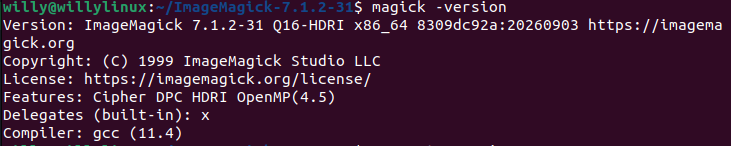
\includegraphics[width=0.9\linewidth]{assets/magick_version.png}
    \caption{Verification of the installed ImageMagick version.}
\label{fig:imagemagick-version}
\end{figure}

Several command-line operations were performed in order to become familiar with the main ImageMagick functionalities. First, an example image was generated using one of the images included with ImageMagick:

\begin{verbatim} magick logo: original.png \end{verbatim}

Information about the image, such as its dimensions, format, color space, and bit depth, can be obtained with the \texttt{identify} command:

\begin{verbatim} magick identify original.png \end{verbatim}

\begin{figure}[H]
    \centering
    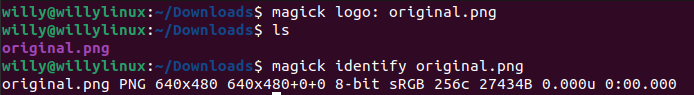
\includegraphics[width=0.9\linewidth]{assets/basic1.png}
    \caption{Basic commands 1.}
    \label{fig:commands1}
\end{figure}

ImageMagick can then apply a wide variety of transformations. Some of the operations tested were resizing, rotation, grayscale conversion, cropping, and blurring:

\begin{verbatim}
magick <input> -resize 50% <output>
magick <input> -rotate 20 <output>
magick <input> -colorspace Gray <output>
magick <input> -crop 300x200+20+20 <output>
magick <input> -blur 0x3 <output>
\end{verbatim}

\begin{figure}[H]
    \centering
    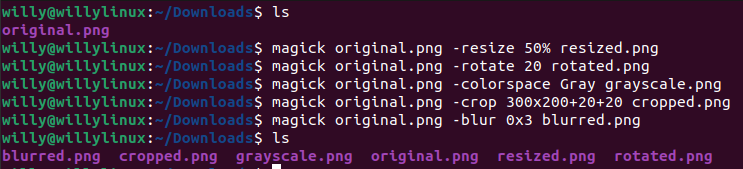
\includegraphics[width=0.9\linewidth]{assets/basic2.png}
    \caption{Basic commands 2.}
    \label{fig:commands2}
\end{figure}

\begin{figure}[H]
    \centering
    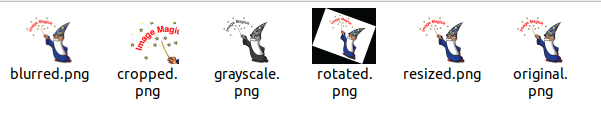
\includegraphics[width=0.9\linewidth]{assets/images_example.png}
    \caption{Example of the images created.}
    \label{fig:exampleimages}
\end{figure}

Figure~\ref{fig:exampleimages} shows the results of these operations. These experiments illustrate that ImageMagick can be used not only for format conversion but also for image transformations, color-space manipulation, filtering, image composition, and image inspection.

The formats supported by the installed version can be inspected with:

\begin{verbatim} magick identify -list format \end{verbatim}

In particular, the output contains the \texttt{AVS} format identified as \emph{AVS X image}, with both reading and writing support \cite{imagemagick_formats}.

\begin{figure}[H]
    \centering
    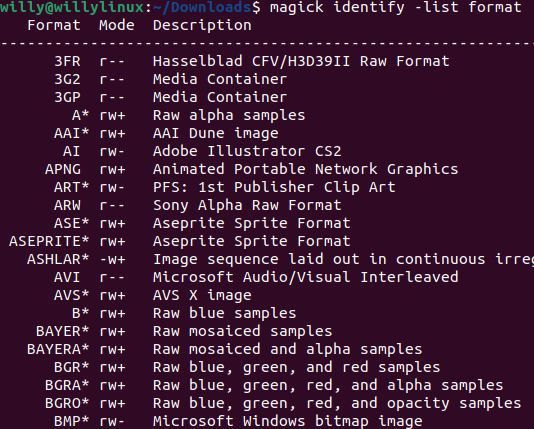
\includegraphics[width=0.7\linewidth]{assets/formats.png}
    \caption{Example of some formats in Image Magick.}
    \label{fig:imagemagick_formats}
\end{figure}

%==================================================================================

\section{ImageMagick: AVS Format}

ImageMagick identifies the \texttt{AVS} format as the \emph{AVS X image} format and provides both reading and writing support for it \cite{imagemagick_formats}. The format should not be confused with video formats that use the same AVS acronym.

The AVS X-Image format originated on UNIX workstations and was commonly used to represent true-color raster images with transparency information. Each pixel contains four 8-bit components, giving a total of 32 bits, or four bytes, per pixel \cite{goldensoftware_avs}. The four components are stored in the order alpha, red, green, and blue (A-R-G-B) \cite{bourke_avs,imagemagick_avs_source}.

The internal structure of a single AVS X-Image is particularly simple. The file begins with an 8-byte header followed immediately by the raster pixel data \cite{bourke_avs}. The header contains two unsigned 32-bit integers representing the image width and height. Both integers are stored using most-significant-byte-first, or big-endian, byte ordering \cite{imagemagick_avs_source}.

Pixels are stored from left to right and from the top of the image to the bottom \cite{bourke_avs}. For each pixel, one unsigned byte is stored for each of the four components: a == alpha, r == red, g = reen, b == blue, where each colour/alpha component is 1 unsigned byte \cite{bourke_avs}.

Unlike formats such as PNG or JPEG, the basic AVS X-Image representation does not contain a complex metadata structure or compressed image stream. ImageMagick's AVS encoder writes the width (the first four bytes) and height (the next four bytes) directly, followed by the four channel bytes for every pixel \cite{imagemagick_avs_source}.

For example, to verify the internal structure of the AVS format, the image show next will be converted from JPEG to AVS using ImageMagick.

\begin{figure}[H]
    \centering
    
\includegraphics[width=0.35\linewidth]{assets/smiley.jpg}
    \caption{Original image used for the AVS format experiment.}
    \label{fig:smiley-original}
\end{figure}

The image can be converted to .avs using:
\begin{verbatim} magick smiley.jpg smiley.avs \end{verbatim}

\begin{figure}[H]
    \centering
    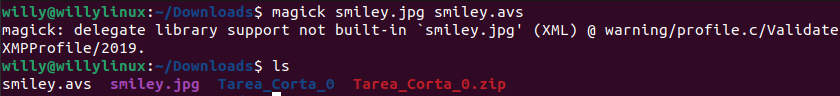
\includegraphics[width=0.9\linewidth]{assets/smiley_converted.png}
    \caption{Image in .avs format.}
    \label{fig:smiley-original}
\end{figure}

The original image has a resolution of $612 \times 612$ pixels. The first bytes of the resulting AVS file can be examined with:

\begin{verbatim} xxd -g 1 -l 32 smiley.avs \end{verbatim}

Since 612 in hexadecimal is \texttt{0x264}, its 32-bit big-endian
representation is 00 00 02 64. Therefore, the first eight bytes of the AVS file are: 00 00 02 64  00 00 02 64.

\begin{figure}[H]
    \centering
    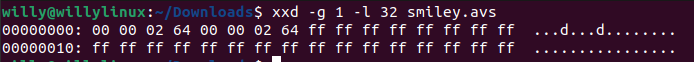
\includegraphics[width=0.9\linewidth]{assets/smiley_stats.png}
    \caption{Bytes in a .avs format.}
    \label{fig:smiley-original}
\end{figure}

As a matter of fact, the term AVS is also associated with scientific-visualization formats that should not be confused with AVS X-Image. In particular, AVS Field files, commonly identified by the \texttt{.fld} extension, are designed to describe multidimensional scientific datasets rather than ordinary two-dimensional raster images.

Scientific-visualization research such as the work of Nonaka et al. discusses visualization of large-scale datasets on high-performance computing systems \cite{nonaka2018sparc64fx}. Such scientific data representations serve a different purpose from the AVS X-Image format implemented by ImageMagick.



%==================================================================================
\section{Load Matrix with .avs}
The function \texttt{load\_avs} reads an AVS file and returns a matrix of pixels in memory.

As explained earlier, the AVS format stores the image width and height in the first eight bytes of the file, followed by the pixel data. The function reads this information and allocates memory for a matrix of pixels.

Given that we are working in a little-endian architecture, the function must convert the big-endian bytes of the header to little-endian integers.

First of all, we have to define a structure to represent a pixel in memory:

\begin{lstlisting}
typedef struct {
    unsigned char a; // alpha channel
    unsigned char r; // red channel
    unsigned char g; // green channel
    unsigned char b; // blue channel
} Pixel;
\end{lstlisting}

This structure allows us to store the four channels of a pixel in a single object. 

To start loading the image, we open the AVS file in binary read mode, then we read the first four bytes to obtain the image width, and the next four bytes to obtain the image height. We convert these bytes from big-endian to little-endian integers.

\begin{lstlisting}
    FILE *file = fopen(filename, "rb"); // read file as binaries

    if (file == NULL) {
        printf("No file found.\n");
        return NULL;
    }

    // define a 4 bytes buffer to read the header
    unsigned char buffer[4];

    // read first 4 bytes of the header -> width
    fread(buffer, 1, 4, file);

    // arrange big endian bytes to little endian
    width = ((int)buffer[0] << 24) |
            ((int)buffer[1] << 16) |
            ((int)buffer[2] << 8) |
            buffer[3];

    // read the follwing 4 bytes -> height
    fread(buffer, 1, 4, file);

    // arrange header big endian bytes to little endian
    height = ((int)buffer[0] << 24) |
            ((int)buffer[1] << 16) |
            ((int)buffer[2] << 8) |
            buffer[3];
\end{lstlisting}

After obtaining the dimensions, we allocate memory for a matrix of pixels with the specified width and height. 

\begin{lstlisting}
    Pixel **image = malloc(height *sizeof(Pixel *));

    for (int y=0; y < height; y++) {
        // for every y in height, create row
        image[y] = malloc(width * sizeof(Pixel));
    }
\end{lstlisting}

We then read the pixel data from the file, storing each pixel in the corresponding position in the matrix.

\begin{lstlisting}
    for (int y = 0; y < height; y++) {
        for (int x = 0; x < width; x++) {
            fread(buffer, 1, 4, file);
            image[y][x].a = buffer[0];
            image[y][x].r = buffer[1];
            image[y][x].g = buffer[2];
            image[y][x].b = buffer[3];
        }
    }
\end{lstlisting}


Finally, we close the file and return the pointer to the matrix of pixels.


\section{Save .avs from memory}

The function \texttt{save\_avs} stores an image represented in memory as an AVS
file. Its declaration is:

\begin{lstlisting}
int save_avs(const char *filename, Pixel **image,
             int image_width, int image_height)
\end{lstlisting}

The function receives the output filename, a matrix of pixels, the image width,
and the image height. It returns \texttt{0} if the operation is successful and
\texttt{-1} if an error occurs.

\subsection{Opening the output file}

The file is opened in binary write mode:

\begin{lstlisting}
FILE *file = fopen(filename, "wb");
\end{lstlisting}

The \texttt{w} flag enables writing, while the \texttt{b} flag indicates that
the file must be treated as binary data. If the file cannot be created, the
function reports the error and returns \texttt{-1}.

\begin{lstlisting}
if (file == NULL) {
    printf("Could not create file.\n");
    return -1;
}
\end{lstlisting}

\subsection{Writing the image width}

The AVS format stores the width in the first four bytes of the file. These bytes
must be written in big-endian order. The bit-shift operators extract each byte
from the integer:

\begin{lstlisting}
buffer[0] = (unsigned char)((image_width >> 24) & 0xff);
buffer[1] = (unsigned char)((image_width >> 16) & 0xff);
buffer[2] = (unsigned char)((image_width >> 8) & 0xff);
buffer[3] = (unsigned char)(image_width & 0xff);
\end{lstlisting}

The four bytes are then written to the file using \texttt{fwrite}:

\begin{lstlisting}
if (fwrite(buffer, 1, 4, file) != 4) {
    fclose(file);
    return -1;
}
\end{lstlisting}

The return value of \texttt{fwrite} is checked to ensure that all four bytes
were written successfully.

\subsection{Writing the image height}

The height is written using the same big-endian conversion:

\begin{lstlisting}
buffer[0] = (unsigned char)((image_height >> 24) & 0xff);
buffer[1] = (unsigned char)((image_height >> 16) & 0xff);
buffer[2] = (unsigned char)((image_height >> 8) & 0xff);
buffer[3] = (unsigned char)(image_height & 0xff);
\end{lstlisting}

The resulting four bytes are written immediately after the width.
The first eight bytes of the AVS file contain the image dimensions:

\begin{verbatim}
4 bytes for the width
4 bytes for the height
\end{verbatim}

\subsection{Writing the pixel data}

After writing the header, the function iterates through every row and column of
the image:

\begin{lstlisting}
for (int y = 0; y < image_height; y++) {
    for (int x = 0; x < image_width; x++) {
\end{lstlisting}

Each pixel is stored in the order alpha, red, green, and blue:

\begin{lstlisting}
buffer[0] = image[y][x].a;
buffer[1] = image[y][x].r;
buffer[2] = image[y][x].g;
buffer[3] = image[y][x].b;
\end{lstlisting}

Each pixel occupies four bytes in the output file. The function writes those
bytes and verifies that the operation succeeds:

\begin{lstlisting}
if (fwrite(buffer, 1, 4, file) != 4) {
    fclose(file);
    return -1;
}
\end{lstlisting}

Pixels are written from left to right and from the top row to the bottom row.

\subsection{Closing the file}

Once the header and all pixel data have been written, the file is closed:

\begin{lstlisting}
if (fclose(file) != 0) {
    return -1;
}
\end{lstlisting}

If the file is closed successfully, the function returns zero:

\begin{lstlisting}
return 0;
\end{lstlisting}

\subsection{Using the function in \texttt{main}}

The image is first loaded into memory using \texttt{load\_avs}:

\begin{lstlisting}
Pixel **image = load_avs("image.avs");
\end{lstlisting}

The in-memory image is then saved as a new AVS file:

\begin{lstlisting}
if (save_avs("image_copy.avs", image, width, height) == 0) {
    printf("Image saved successfully.\n");
} else {
    printf("Could not save image.\n");
}
\end{lstlisting}

This creates \texttt{image\_copy.avs} with the same dimensions and pixel values
as the original image.

Finally, the memory allocated for the pixel matrix is released row by row:

\begin{lstlisting}
for (int y = 0; y < height; y++) {
    free(image[y]);
}
free(image);
\end{lstlisting}

This prevents memory leaks after the image has been saved.



\bibliographystyle{IEEEtran}
\bibliography{ref}

\end{document}